\section{Generative adversarial network}
Generative Adversarial Networks (GANs) represent a powerful class of deep learning models comprising generator(s) ($G$) and discriminator(s) ($D$). They are fully connected layers which often consist of deep convolutional neural networks (CNNs). \cite{siahkoohi2018seismic} $G$ generates synthetic samples from the embedding space while $D$ distinguishes between generated and real dataset samples. Through iterative training epochs, both $G$ and $D$ evolve by minimizing their respective losses, fostering the generation of more realistic samples by the generator.

\begin{figure}[H]
    \centering
    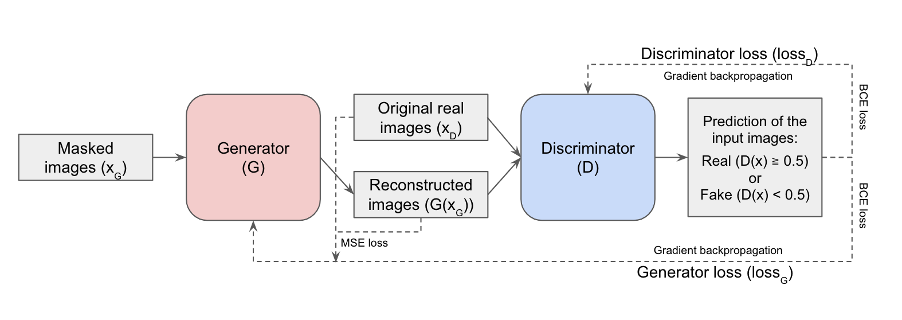
\includegraphics[width=\textwidth]{Figure/Front_page/flow chart.png}
    \caption{\textit{GAN architecture (modified from \cite{saxena2021generative})}}
    \label{fig:archi}
\end{figure}

\noindent In the context of image reconstruction, our application involves presenting $G$ with images containing missing columns, denoted as $x_{G}$, and obtaining interpolated images as the output, i.e., $G(x_{G})$. Subsequently, the discriminator $D$ assesses whether the given sample is a reconstructed image ($G(x_{G})$) or an authentic dataset image ($x_{D}$), assigning a scalar value between 0 (indicating a reconstructed image) and 1 (indicating a real dataset image). The generator loss ($loss_{G}$) is computed through a combination of binary cross-entropy (BCE) loss between $D(G(x_{G}))$ and 1, as well as mean squared error (MSE) loss between $G(x_{G})$ and $x_{D}$ (Equation \ref{eq:loss_G}). In contrast, the discriminator loss ($loss_{D}$) is determined by the sum of binary cross-entropy (BCE) loss between $D(x_{D})$ and 1, along with binary cross-entropy (BCE) loss between $D(G(x_{G}))$ and 0. (Equation 
 \ref{eq:loss_D}) The gradients of these losses are backpropagated to update the parameters of $G$ and $D$ \cite{saxena2021generative}.

\begin{equation}
loss_{G} = \underbrace{loss_{BCE}(D(G(x_{G})),1)}_\text{$G$ performance on producing synthetic image} + \underbrace{loss_{MSE}(G(x_{G}),x_{D})}_\text{Difference between synthetic and real image}
\label{eq:loss_G}
\end{equation}
\begin{equation}
loss_{D} = (\underbrace{loss_{BCE}(D(x_{D}),1)}_\text{$D$ performance on classifying real image} + \underbrace{loss_{BCE}(D(G(x_{G})),0)}_\text{$D$ performance on classifying synthetic image})/2
\label{eq:loss_D}
\end{equation}
 
\section{Neural network architecture}
Neural networks (NN) comprise interconnected layers of neurons, with various layer types (e.g., convolution, linear, and pooling) and activation functions (e.g., Rectified Linear Unit (ReLU), sigmoid, and tanh). The architecture's complexity impacts image reconstruction performance and computation time. Three neural network architectures have been investigated on our generator and discriminator, incorporating refined hyperparameters.

\begin{figure}[H]
    \centering
    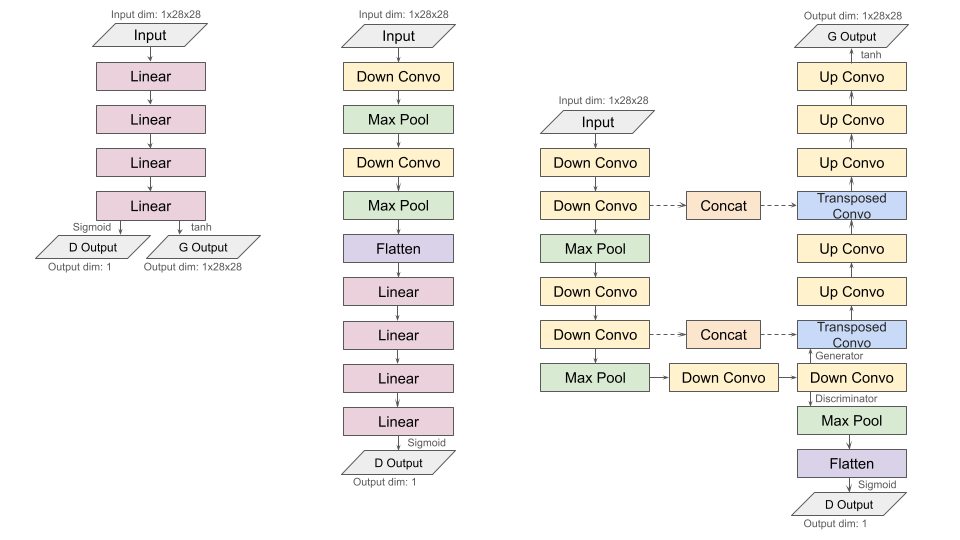
\includegraphics[width=\textwidth]{Figure/Front_page/Network architecture.png}
    \caption{\textit{Neural network architecture of linear layer model (left), LeNeT-5 (center) and U-NET (right)}}
    \label{fig:archi}
\end{figure}

\subsection{Linear layer model} \label{sub:linear}
This is the simplest model we built for this study, which consists of four linear transformations $y=xA^{T}+b$ and three ReLU functions. (Figure \ref{fig:archi} left) ReLU functions introduce non-linearity to NN, enabling them to learn complex tasks and mitigating the vanishing gradient problem. The generator employs linear layers with an increased output dimension, while the discriminator utilizes linear layers with a decreased output dimension.

\subsection{LeNeT-5}\label{sub:lenet}
Proposed in 1988, LeNet-5 stands as one of the earliest convolutional neural network (CNN) architectures \cite{lecun1998gradient}, notably designed for handwritten digit recognition. It is composed of two convolutional and pooling layers, a flattening function, four linear transformations, and three ReLU functions. (Figure \ref{fig:archi} center) 
Convolutional layers apply a kernel to each image pixel, capturing local patterns, while pooling layers retain the most relevant "summary" of features by downsampling the information. As LeNeT-5 down-samples the input dimension to 1, i.e. for classification purposes, we applied LeNet-5 only to our discriminator.

\subsection{U-NET}\label{sub:unet}
Introduced in 2015 by Olaf Ronneberger, Philipp Fischer, and Thomas Brox, U-NET is a convolutional neural network (CNN) architecture specifically designed for image segmentation tasks. Its distinctive U-shaped architecture comprises two key segments: the contracting path and the expanding path. \cite{ronneberger2015u, long2015fully}
\\\\
In our generator model, inspired by U-NET, the contracting path is implemented with six convolutional and two pooling layers. This configuration aims to decrease the spatial resolution of the input image while simultaneously increasing the number of feature channels. (Figure \ref{fig:archi} right) The contracting path is responsible for extracting essential features from the input image.
\\\\
Conversely, the expanding path in our model incorporates two transposed convolutional, five convolutional layers, and two concatenation layers.  (Figure \ref{fig:archi} right) This part of the network is designed to elevate the spatial resolution of the feature maps. Additionally, it combines these features with information from the contracting path to generate the final segmentation mask, using the concatenate functions.
\\\\
In our discriminator model, we leveraged the contracting path of the U-Net architecture, augmenting it with one pooling layer, one flattening function, and one linear layer. Our experimentation revealed that the U-Net architecture yielded the most refined interpolation results, which will be further discussed in chapter \ref{ch:4}.

